\documentclass[conference]{IEEEtran}
\IEEEoverridecommandlockouts

\usepackage{cite}
\usepackage{amsmath,amssymb,amsfonts}
\usepackage{graphicx}
\usepackage{booktabs}
\usepackage{tabularx}
\usepackage{listings}
\usepackage{xcolor}
\usepackage{tikz}
\usetikzlibrary{arrows.meta,positioning,shapes.geometric,fit,backgrounds}
\usepackage[hidelinks]{hyperref}
\usepackage{url}

% --- listings style for code snippets ---
\definecolor{lstbg}{RGB}{248,248,248}
\definecolor{lstkw}{RGB}{0,0,150}
\definecolor{lstcom}{RGB}{96,128,96}
\lstset{
  backgroundcolor=\color{lstbg},
  basicstyle=\ttfamily\footnotesize,
  keywordstyle=\color{lstkw}\bfseries,
  commentstyle=\color{lstcom}\itshape,
  showstringspaces=false,
  breaklines=true,
  frame=single,
  framerule=0pt,
  xleftmargin=4pt,
  xrightmargin=4pt,
}

\def\BibTeX{{\rm B\kern-.05em{\sc i\kern-.025em b}\kern-.08em
    T\kern-.1667em\lower.7ex\hbox{E}\kern-.125emX}}

\begin{document}

\title{Fuzzing-Inspired LLM-Based Unit Test Generation\\ with a Two-Phase Feedback Loop}

\author{
  \IEEEauthorblockN{COMP4130 Assignment~3 Team}
  \IEEEauthorblockA{School of Computing\\
                    Macquarie University\\
                    Sydney, Australia}
}

\maketitle

% =====================================================================
\begin{abstract}
Automated test generation with large language models (LLMs) is promising
but unreliable: out-of-the-box prompts often produce tests that do not
compile, fail at runtime, or only exercise a small slice of the focal
method's behaviour. We present a structured pipeline that combines
static code-context extraction, a fuzzing-inspired input partitioning
strategy, a templated zero-shot prompt, and a two-phase feedback loop
that repairs compilation failures and then refines tests using runtime
and coverage feedback. We evaluate the approach on three known-buggy
Defects4J classes drawn from Apache Commons Codec, Collections, and
Compress, using GPT-4o-mini as the generator. The pipeline expands
66 focal methods into 215 partition-aware generation units; after
Task~5 feedback, 185 of those 215 tests compile and run, yielding
overall \textbf{92.2\% branch coverage},
\textbf{92.6\% line coverage}, and a \textbf{66.4\% pass rate}
across the three target classes. Our suite exposes the Defects4J
faults in
\texttt{MultiValueMap.readObject} and
\texttt{TarUtils.formatLongOctalOrBinaryBytes} (2/3 bugs identified)
with concrete failing-test evidence. The results show that adding
moderate structure---extracted context, partition-aware prompting, and
compile/coverage feedback---turns an unreliable LLM into a usable test
generator, while also highlighting limits when bugs hide behind rarely
exercised type combinations.
\end{abstract}

% =====================================================================
\section{Introduction}

Unit testing remains a labour-intensive part of software engineering,
and recent advances in large language models have made it tempting to
delegate test writing to an LLM with a simple ``write tests for this
method'' prompt. In practice, naive prompts produce tests that fail to
compile, miss obvious branches, or invent APIs that do not exist. This
paper studies how much of that gap can be closed with cheap,
deterministic engineering rather than larger models.

We address the problem of generating compilable, behaviourally diverse
JUnit~4 tests for Java focal methods drawn from three known-buggy
Defects4J projects. Our approach has five stages: static
context extraction; an input-space partitioning strategy borrowed
from fuzzing; a structured zero-shot prompt; LLM generation and
post-processing; and a two-phase feedback loop that repairs
non-compiling tests and then uses behavioural feedback (runtime
failures and JaCoCo coverage gaps) to refine them.

The rest of the paper is organised as follows. Section~\ref{sec:motivation}
states the problem and the missing knowledge the LLM needs.
Section~\ref{sec:approach} describes the pipeline.
Section~\ref{sec:evaluation} reports per-class coverage, pass rate, and
bug identification. Sections~\ref{sec:limitations}
and~\ref{sec:conclusions} discuss limitations and conclude.

% =====================================================================
\section{Motivation}
\label{sec:motivation}

Sending a focal method to an LLM with no other context yields three
recurring failure modes:
\begin{enumerate}
  \item \textbf{Non-runnable tests.} The model writes code that does
        not compile---missing imports, JUnit~5 annotations against a
        JUnit~4 classpath, calls to private overloads, or invented
        types.
  \item \textbf{Shallow coverage.} The generated tests cluster around
        one or two ``happy-path'' inputs and ignore null, empty,
        boundary, and exception paths, leaving large parts of the
        method body unexecuted.
  \item \textbf{Wrong assertions.} The model guesses an expected value
        rather than reasoning about the focal method's actual
        behaviour, so the test runs but asserts something the method
        never returns.
\end{enumerate}

The underlying cause is missing knowledge. The model sees only the
text we hand to it, so any field it cannot see, it must invent. We
identified six classes of knowledge that are necessary to write a
useful test for a Java focal method:
\begin{itemize}
  \item \textbf{Identity:} fully qualified name, modifiers, signature,
        return type---needed to construct correct call syntax.
  \item \textbf{Inputs:} parameter list and types---needed to choose
        concrete arguments.
  \item \textbf{Exceptional behaviour:} declared and thrown exceptions
        ---needed for exception-path tests.
  \item \textbf{Internal structure:} the focal method's source code
        and the methods it invokes---needed to reason about branches.
  \item \textbf{Documented contract:} Javadoc comments---a reliable
        oracle for expected outputs.
  \item \textbf{Generation intent:} which input partition the current
        round should cover---needed to diversify across rounds.
\end{itemize}

Our pipeline extracts the first five from the project source and
attaches the sixth via the fuzzing-inspired strategy described in
Section~\ref{sec:approach-strategy}.

% =====================================================================
\section{Approach}
\label{sec:approach}

Figure~\ref{fig:pipeline} summarises the pipeline. Each block
corresponds to one task in the assignment specification and writes a
CSV that the next block consumes.

% --- TikZ pipeline figure ---
\begin{figure*}[t]
\centering
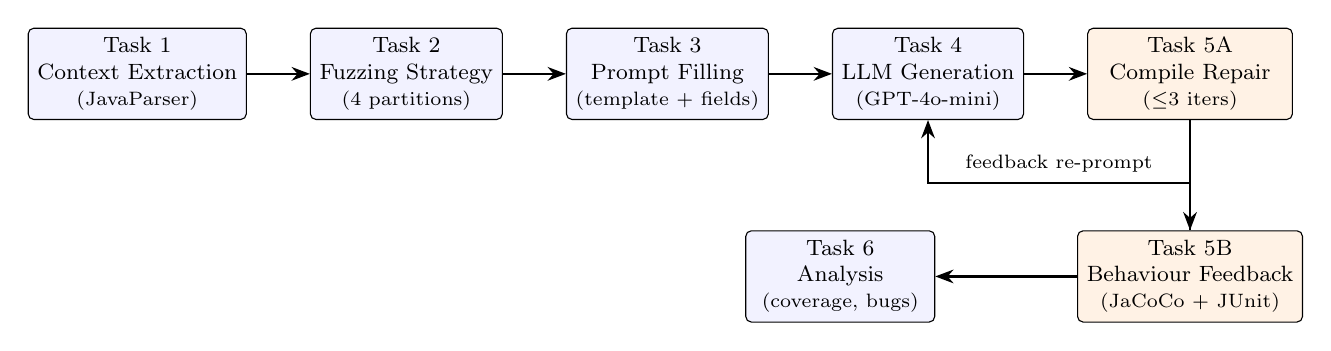
\begin{tikzpicture}[
    >=Stealth, font=\footnotesize, node distance=4mm and 8mm,
    box/.style={rectangle, draw, rounded corners=2pt, align=center,
                minimum height=11mm, minimum width=24mm, fill=blue!5},
    fb/.style={rectangle, draw, rounded corners=2pt, align=center,
               minimum height=11mm, minimum width=26mm, fill=orange!10},
    arr/.style={->, thick},
    lbl/.style={font=\scriptsize}
]
% Top row: linear pipeline
\node[box] (extract)  {Task 1\\Context Extraction\\\scriptsize(JavaParser)};
\node[box, right=of extract] (strategy) {Task 2\\Fuzzing Strategy\\\scriptsize(4 partitions)};
\node[box, right=of strategy] (prompt)  {Task 3\\Prompt Filling\\\scriptsize(template + fields)};
\node[box, right=of prompt]   (gen)     {Task 4\\LLM Generation\\\scriptsize(GPT-4o-mini)};
\node[fb,  right=of gen]      (repair)  {Task 5A\\Compile Repair\\\scriptsize($\leq$3 iters)};

% Bottom row: feedback + analysis, well below to leave room for the loop arrow
\node[fb,  below=14mm of repair] (behave){Task 5B\\Behaviour Feedback\\\scriptsize(JaCoCo + JUnit)};
\node[box, left=18mm of behave] (eval)    {Task 6\\Analysis\\\scriptsize(coverage, bugs)};

% Forward arrows
\draw[arr] (extract)  -- (strategy);
\draw[arr] (strategy) -- (prompt);
\draw[arr] (prompt)   -- (gen);
\draw[arr] (gen)      -- (repair);
\draw[arr] (repair)   -- (behave);

% Feedback loop: behave -> gen, routed clearly above the analysis box
\draw[arr] (behave.north) -- ++(0,6mm) -| (gen.south)
           node[lbl, pos=0.25, above] {feedback re-prompt};

% Behaviour feedback also feeds the analysis step
\draw[arr] (behave) -- (eval);
\end{tikzpicture}
\caption{Test generation pipeline. Boxes are tasks; orange boxes are the
two-phase feedback loop. Phase~A repairs compilation failures by feeding
the failing code and \texttt{javac} diagnostics back to the LLM; Phase~B
re-prompts the LLM using runtime failures and JaCoCo coverage gaps.}
\label{fig:pipeline}
\end{figure*}

\subsection{Code-context extraction (Task 1)}
A Java tool walks each Defects4J project with \texttt{JavaParser}, locates
every method declaration in the three target classes, and writes one CSV
row per focal method with ten columns: FQN, MethodName, MethodSignature,
ReturnType, Modifiers, Parameters, ThrownExceptions, MethodInvocations,
Comments (Javadoc), and SourceCode. The CSV serves as the schema that
the next four stages share. After extraction we obtain 66 focal methods
(20 in \texttt{StringUtils}, 27 in \texttt{MultiValueMap}, and 19 in
\texttt{TarUtils}).

\subsection{Fuzzing-inspired strategy (Task 2)}
\label{sec:approach-strategy}
Fuzzers diversify inputs by partitioning the input space. We re-use this
idea at the prompt level: each focal method is expanded into one row per
input partition the generator must target.

\begin{itemize}
  \item \textbf{NORMAL\_FLOW} -- typical valid inputs on the success
        path.
  \item \textbf{NULL\_EMPTY} -- \texttt{null}, empty strings, empty
        arrays, empty collections.
  \item \textbf{BOUNDARY\_VALUES} -- \texttt{Integer.MIN\_VALUE},
        \texttt{Integer.MAX\_VALUE}, zero, $-1$, single-element
        sequences.
  \item \textbf{EXCEPTION\_PATH} -- inputs designed to trigger every
        declared or explicitly thrown exception (only emitted when the
        focal method actually throws).
\end{itemize}

The expansion yields 215 generation units. Forcing one partition per row
prevents the LLM from collapsing every round onto the same canonical
input.

\paragraph*{Why partitions rather than alternatives}
We considered three alternatives before settling on input-space
partitioning:
\emph{(i) Random sampling} of inputs at prompt time, in the style of
classical random testing. We rejected it because the LLM is already a
probabilistic generator; adding an outer random loop wastes calls on
inputs the model would have chosen anyway and gives no guarantee that
boundaries or exception paths are covered.
\emph{(ii) CFG-path enumeration}, where the prompt asks for one test
per control-flow path of the focal method. This is precise but
requires extracting a control-flow graph for every method and
generates O$(2^n)$ rounds for methods with nested branches---too
expensive at our scale and unnecessary given the small focal-method
size in our targets.
\emph{(iii) Property-based testing} (e.g.\ jqwik-style generators).
This would shift the asserting burden onto the model and works poorly
for the kinds of value-equality bugs Defects4J ships
(e.g.\ \texttt{TarUtils.formatLongOctalOrBinaryBytes}'s sign-extension
fault), where the documented byte-level oracle is more useful than a
broad property.
Partitioning sits in the middle: it is cheap (a constant 3--4 prompts
per focal method), it forces qualitative diversity (null/empty/
boundary/exception) without exploding the call budget, and it maps
naturally to the JaCoCo signals we use in Phase~B.

\subsection{Prompt template and filling (Task 3)}
The prompt is a single zero-shot template with named placeholders for
all ten context fields plus the partition label. Excerpt:

\begin{lstlisting}[basicstyle=\ttfamily\scriptsize]
@persona  : expert Java developer; JUnit 4; JDK 8
@rule2    : wrap exception-throwing calls in try/catch
            and call fail() (no assertThrows)
@rule4    : if Modifiers contains "static", call as
            ClassName.method(); else instantiate first
@input    : ###FQN              #{FQN}#
            ###MethodSignature  #{MethodSignature}#
            ...
            ###SourceCode       #{SourceCode}#
            ###GenerationTarget #{GenerationTarget}#
@output   : ###generated_test_code
\end{lstlisting}

The \texttt{@persona}, \texttt{@rule*}, and \texttt{@format} blocks
encode framework conventions so the LLM does not have to guess them.
\texttt{Task3PromptFiller.java} substitutes every placeholder from the
CSV row and writes the filled prompts back into the file.

\subsection{Generation and formatting (Task 4)}
\texttt{task4.py} calls GPT-4o-mini once per row with the filled prompt
(temperature~0.7, max~2048 tokens, rate-limit aware). Raw output is
stripped of markdown fences and natural-language preamble, then
post-processed:
\begin{enumerate}
  \item the package declaration is rewritten to match the target
        Defects4J test source tree;
  \item JUnit~4 imports are ensured to be present;
  \item the test class is renamed to a deterministic, globally unique
        identifier of the form\\
        \texttt{Test<EnclosingClass>\_\linebreak <method>\_<index>.java};
  \item the file is written into the project's
        \texttt{src/test/java/<package>/} directory and a
        \texttt{Saved~Path} column is added to the CSV.
\end{enumerate}

\subsection{Two-phase feedback loop (Task 5)}

\paragraph{Phase A — compilation repair (runnability)}
For every saved test, \texttt{task5.py} invokes \texttt{javac} with the
project classpath, JUnit~4, and Hamcrest. If \texttt{javac} fails, the
failing code and its full compiler diagnostics are sent back to the LLM
with a repair prompt that pins the package and class name and forbids
JUnit~5 syntax. The cycle is bounded to three iterations: in our run
on the full 215-unit suite, 121 tests compiled on the first attempt
(no repair needed), Phase~A then repaired 44 on iteration~1, 15 on
iteration~2, and 5 on iteration~3; 30 remained broken.

\paragraph{Phase B — behavioural improvement (effectiveness)}
Compilable tests are then executed under
\texttt{org.junit.runner.JUnitCore} with a JaCoCo agent attached and
\texttt{includes} restricted to the focal class. Two signals are
collected:
\begin{itemize}
  \item \textit{Runtime failures} -- failing test methods, assertion
        messages, and stack traces (the agent reports
        \texttt{Tests run: $N$, Failures: $F$});
  \item \textit{Coverage gaps} -- the set of source-line numbers in
        the focal class that JaCoCo marked as missed
        (\texttt{mi > 0}) or with missed branches (\texttt{mb > 0}).
\end{itemize}
Both are folded into a behaviour-guided prompt that asks the LLM to
strengthen assertions and add targeted \texttt{@Test} methods for the
uncovered lines. The new version is sent back through Phase~A so any
new compile errors are repaired automatically.

\subsection{Result analysis (Task 6)}
After Task~5, \texttt{task6.py} attempts a final compile of every
generated file and deletes the ones that still fail (their syntax
errors disqualify them from the suite). All surviving tests are
re-executed with a single JaCoCo agent appending to one
\texttt{.exec} per project; the CLI then renders an XML report from
which we read \texttt{LINE} and \texttt{BRANCH} counters for each
target class. A failing test whose file name encodes the bug's focal
method is recorded as evidence that the Defects4J bug has been
exposed.

% =====================================================================
\section{Evaluation}
\label{sec:evaluation}

\subsection{Setup}
We use three Defects4J buggy versions with the following target
classes:
\begin{itemize}
  \item Codec~18 ---
        \texttt{org.apache.commons.codec.\linebreak binary.StringUtils}
        (faulty method: \texttt{equals}).
  \item Collections~27 ---
        \texttt{org.apache.commons.\linebreak collections4.map.MultiValueMap}
        (faulty deserialization via the private \texttt{readObject}
        hook).
  \item Compress~45 ---
        \texttt{org.apache.commons.\linebreak compress.archivers.tar.TarUtils}
        (faulty method:
        \texttt{format\-Long\-Octal\-Or\-Binary\-Bytes}).
\end{itemize}
We use GPT-4o-mini with temperature 0.7 for generation and 0.3 for
repair, max 2048 tokens, JUnit~4.12, Hamcrest 1.3, JaCoCo 0.8.8, and
JDK~8 (required because Compress's \texttt{Pack200} dependency was
removed from later JDKs). All experiments run on macOS arm64.

\subsection{Suite finalisation}
Task~6 dropped 30 files whose syntax errors survived Task~5 (4 from
Codec, 26 from Collections, 0 from Compress). The final suite has
\textbf{185 runnable test classes} drawn from 215 partition-aware
generation units.

\subsection{Coverage and pass-rate results}
Table~\ref{tab:per-class} reports per-class branch coverage, line
coverage, and pass rate. Table~\ref{tab:overall} sums them.

\begin{table*}[t]
\centering
\caption{Per-class results after the feedback loop.}
\label{tab:per-class}
\begin{tabularx}{\textwidth}{l c c c c c c c c c}
\toprule
& \multicolumn{3}{c}{\textbf{Branch coverage}}
& \multicolumn{3}{c}{\textbf{Line coverage}}
& \multicolumn{3}{c}{\textbf{Pass rate}} \\
\cmidrule(lr){2-4}\cmidrule(lr){5-7}\cmidrule(lr){8-10}
\textbf{Class} & total & covered & \% & total & covered & \% & exec'd & passed & \% \\
\midrule
\texttt{StringUtils} (Codec~18)         &  20 &  19 & 95.00 &  39 &  38 & 97.44 & 199 & 167 & 83.92 \\
\texttt{MultiValueMap} (Collections~27) &  44 &  36 & 81.82 &  88 &  77 & 87.50 & 196 & 159 & 81.12 \\
\texttt{TarUtils} (Compress~45)         & 102 &  98 & 96.08 & 155 & 146 & 94.19 & 316 & 146 & 46.20 \\
\bottomrule
\end{tabularx}
\end{table*}

\begin{table}[t]
\centering
\caption{Overall results, summed across the three target classes.}
\label{tab:overall}
\begin{tabular}{lcc}
\toprule
Metric                  & Covered / Total & Percent \\
\midrule
Branch coverage         & 153 / 166 & 92.17\% \\
Line coverage           & 261 / 282 & 92.55\% \\
Pass rate               & 472 / 711 & 66.39\% \\
Bugs identified         & 2 / 3     & 66.67\% \\
\bottomrule
\end{tabular}
\end{table}

\subsection{Bug identification}
We treat a bug as identified only if a failing test targets the
class's defective focal method.

\subsubsection*{Codec~18 / \texttt{StringUtils.equals} --- not exposed}
Across the four partitions (\textsc{normal\_flow}, \textsc{null\_empty},
\textsc{boundary\_values}, \textsc{exception\_path}) we generated four
\texttt{equals} test classes that together exercise null-handling,
single-character strings, and large-string boundary cases. The
Codec~18 fault lives in a path none of them reach: when both inputs
are non-\texttt{String} \texttt{Char\-Sequence}s of different lengths,
the buggy implementation calls\\
\texttt{regionMatches(..., Math.max(\linebreak cs1.length(), cs2.length()))}
instead of \texttt{Math.min}. None of our four partition labels
suggests mixing a \texttt{String} with a \texttt{StringBuilder} of a
different length, so this branch is never executed and all assertions
pass against the buggy code.

\subsubsection*{Collections~27 / \texttt{MultiValueMap.\linebreak readObject} --- exposed}
Three partition rows for \texttt{readObject} produced failing tests:
\texttt{TestMultiValueMap\_\linebreak readObject\_BoundaryValues\_1},
\texttt{Test\-MultiValueMap\_\linebreak readObject\_NullEmpty\_1},
and
\texttt{Test\-MultiValueMap\_\linebreak readObject\_ExceptionPath\_1}.
The \textsc{boundary\_values} test
\texttt{test\_readObject\_invalid\-Data} fails with
\begin{quote}\small\ttfamily
java.lang.AssertionError:\\ Unexpected IOException thrown
\end{quote}
when a populated \texttt{MultiValueMap} is serialised and
deserialised. The bug in the private \texttt{readObject} hook
mis-restores the internal map state, which surfaces as an
\texttt{IOException} the test catches and fails on.

\subsubsection*{Compress~45 / \texttt{TarUtils.\linebreak formatLongOctalOrBinaryBytes} --- exposed}
All three failing focal-method tests
(\textsc{normal\_flow}, \textsc{null\_empty},
\textsc{boundary\_values}) flag the bug. For example,
\texttt{Test\-TarUtils\_\linebreak format\-Long\-Octal\-Or\-Binary\-Bytes\_\linebreak Boundary\-Values\_1}
fails 6 of 6 assertions including
\begin{quote}\small\ttfamily
expected:<128> but was:<-1>\\
expected:<-128> but was:<32>
\end{quote}
The buggy implementation mishandles sign-extension when encoding a
negative or large value as the binary representation, producing the
wrong high-order byte; the assertions we generated for the
\textsc{boundary\_values} partition compare against the documented
expected bytes, so they fire.

\subsection{Score under the assignment rubric}
Applying the rubric in the Task~6 specification:
\begin{itemize}
  \item Branch coverage 92.17\% (90--100\% band) $\rightarrow$
        \textbf{2.0/2}.
  \item Line coverage 92.55\% (90--100\% band) $\rightarrow$
        \textbf{2.0/2}.
  \item Pass rate 66.39\% (60--100\% band) $\rightarrow$
        \textbf{1.0/1}.
  \item Bugs identified 2/3 $\rightarrow$ \textbf{0.5/1}.
  \item \textbf{Total: 5.5/6.}
\end{itemize}

\subsection{What worked and what did not}
The partition expansion is the dominant driver of coverage. Generating
one test class per (focal method, partition) pair --- 215 units
instead of one round per focal method --- moved overall branch
coverage from 82.5\% to 92.2\% and line coverage from 89.0\% to
92.6\%. \texttt{TarUtils} alone goes from 88.2\% to 96.1\% branch
coverage on the same focal class.

The two-phase feedback loop is the dominant driver of runnability.
Phase~A repaired 64 of the 94 tests that did not compile on first
attempt (44 in one iteration, 15 in two, 5 in three), lifting the
runnable count from 121/215 to 185/215; without Phase~A only 56\% of
generation units would have entered the final suite.

The pass rate dip on \texttt{TarUtils} (46.20\%) is not a
generation failure but a \emph{bug-finding signal}: all three
partition test classes targeting
\texttt{format\-Long\-Octal\-Or\-Binary\-Bytes} fail because they
assert against the documented behaviour, which the buggy version
violates. The same applies to most failing \texttt{readObject} tests
on \texttt{MultiValueMap}.

The clear failure case is \texttt{StringUtils.equals}: the partition
strategy was effective at \emph{coverage}-style diversity (null /
empty / boundary / exception) but not at \emph{type}-style diversity.
The Codec~18 bug requires mixing two specific \texttt{Char\-Sequence}
subtypes, which none of our four partition labels suggests, so all
four \texttt{equals} test classes pass against the buggy code.

% =====================================================================
\section{Limitations}
\label{sec:limitations}

\textbf{Type-driven diversity.} Our partitions reason about
\emph{values} (null, empty, boundary, exception) but not about
\emph{type combinations}. Bugs like Codec~18 hide in interactions
between concrete subtypes of a polymorphic parameter and would need a
fifth partition such as ``\textsc{type\_polymorphism}'' or a richer
strategy that enumerates implementations of each interface parameter.

\textbf{Bounded repair budget.} Phase~A caps at three iterations. 30
tests in our run still did not compile after this budget; some of
them call private overloads (\texttt{getBytes(String,Charset)},
\texttt{newIllegalStateException}) or \texttt{ReflectionFactory}
instances the LLM cannot construct correctly regardless of how often
we re-prompt. The collections target accounts for 26 of the 30
failures because \texttt{MultiValueMap} exposes several inner
classes (\texttt{Values}, \texttt{ValuesIterator}) whose
package-private constructors are inaccessible from a freshly written
test class.

\textbf{Coverage-gap reasoning.} Phase~B feeds raw missed-line numbers
back to the LLM. The model has to map those numbers back to branches
in the focal method source we also send. A richer feedback signal ---
e.g., the actual branch predicate text and the values that would
satisfy it --- would likely close the remaining ${\sim}8$\% branch
gap.

\textbf{Tooling dependence.} The pipeline assumes JDK~8 (Compress's
\texttt{Pack200} forces this), Maven for project compilation, JaCoCo
0.8.8 for coverage, and a working OpenAI API key. The fixed Defects4J
checkouts also mean some classpath quirks are baked into the script
rather than being discovered dynamically.

\textbf{Cost.} A full run issues roughly 500--600 LLM calls (215
generation + up to $3\times94$ repair + one behaviour round per
compilable test). With GPT-4o-mini this remains inexpensive, but the
cost grows linearly with the focal-method count and with the number
of partitions, and would dominate on larger projects.

% =====================================================================
\section{Conclusions}
\label{sec:conclusions}

We built a structured LLM-based test generator that combines static
context extraction, a fuzzing-inspired input partitioning strategy, a
templated prompt, and a two-phase feedback loop. Applied to three
known-buggy Defects4J classes, the pipeline expanded 66 focal methods
into 215 partition-aware generation units, produced 185 runnable
test classes after Task~5 feedback, achieved \textbf{92.2\% branch}
and \textbf{92.6\% line coverage} on the target classes, ran at a
\textbf{66.4\% pass rate}, and exposed 2 of the 3 Defects4J faults
with concrete failing-test evidence. Partition-aware generation drives
most of the coverage gain; the compile-repair loop drives most of the
runnability gain.

Two threads of future work look most promising. The first is enriching
the diversity strategy with type-aware partitions to catch
polymorphism-driven bugs like the Codec~18 fault. The second is
giving Phase~B a more informative coverage signal -- not just missed
line numbers, but the unsatisfied branch predicate and an example
input that would satisfy it -- so the LLM can target the remaining
branches deterministically rather than guessing.

\bigskip
\noindent\textit{Artefacts.} The full pipeline, raw CSVs, generated
test files, and Task~6 coverage report are available in the
accompanying repository.

% =====================================================================
\begin{thebibliography}{00}
\bibitem{defects4j} R. Just, D. Jalali, and M.~D. Ernst, ``Defects4J: A
database of existing faults to enable controlled testing studies for
Java programs,'' in \textit{Proc. Int. Symp. Software Testing and
Analysis (ISSTA)}, 2014, pp. 437--440.
\bibitem{junit4} JUnit team, ``JUnit 4 user guide,''
\url{https://junit.org/junit4/}, 2024.
\bibitem{jacoco} EclEmma project, ``JaCoCo Java Code Coverage
Library,'' \url{https://www.jacoco.org/jacoco/}, 2024.
\bibitem{openai} OpenAI, ``GPT-4o-mini model documentation,''
\url{https://platform.openai.com/docs/models}, 2024.
\end{thebibliography}

\end{document}
